\documentclass[10pt]{article}
\usepackage[margin=1in]{geometry}
\usepackage[T1]{fontenc}
\usepackage{lmodern}
\usepackage{microtype}
\usepackage{amsmath,amssymb}
\usepackage{booktabs}
\usepackage{enumitem}
\usepackage{xcolor}
\usepackage{caption}
\usepackage{tikz}
\usepackage[colorlinks=true,linkcolor=black,citecolor=blue!50!black,urlcolor=blue!50!black]{hyperref}
\newcommand{\T}[2]{#1}  % figure text: \T{English}{Chinese}
% Shared by the English and the Chinese build. Figure text is written as \T{English}{中文};
% each main file defines \T to pick one.
\usetikzlibrary{arrows.meta,positioning,calc,fit,backgrounds}
\definecolor{mainc}{HTML}{6B7280}   % mainline behaviour
\definecolor{offc}{HTML}{C2410C}    % off-mainline behaviour
\definecolor{wfc}{HTML}{15803D}     % workflow
\definecolor{verc}{HTML}{1D4ED8}    % verifier
\definecolor{hidc}{HTML}{9F1239}    % hidden from the system
\tikzset{
  >={Stealth[length=4pt,width=4pt]},
  card/.style={draw=#1, fill=#1!6, rounded corners=2pt, align=left, inner sep=4pt, font={\scriptsize\hyphenpenalty 10000 \exhyphenpenalty 10000 \relax}},
  card/.default=mainc,
  pill/.style={draw=#1, fill=#1!10, rounded corners=6pt, align=center, inner sep=3pt, font=\scriptsize},
  pill/.default=mainc,
  lab/.style={font=\scriptsize\bfseries, text=#1}, lab/.default=black,
  note/.style={font=\scriptsize\itshape, text=mainc, align=center},
}

\newcommand{\sys}{\textsc{ht2wv}}
\newcommand{\todo}[1]{\textcolor{red}{[#1]}}
\setlist{nosep,leftmargin=1.4em}
\captionsetup{font=small,labelfont=bf}

\title{\textbf{HumanTrace2Workflow\&Verifier}\\[2pt]
\large Compiling a Person's Workflows and Their Verifiers from the Access Records They Already Have}
\author{Zhi Zheng\\ \small National University of Singapore \\ \small\emph{Working draft. Results are preliminary: one run per configuration, synthetic samples.}}
\date{}

\begin{document}
\maketitle

\begin{abstract}
People repeat many procedures on a computer, yet handing one of them to an agent still means describing it,
prompting for it, and checking the result by hand. Recent products turn a single recorded demonstration into a
reusable skill, and recent work induces task models from passive traces. Both recover \emph{how} a task is done.
Neither recovers what the person accepts as \emph{done}. We argue that the two are inseparable: there is no best
workflow, only a best workflow under a particular person's acceptance standard, so the object to learn is a pair
(workflow, verifier). The evidence for the verifier does not lie on the main line of a task but beside it, in
corrections, interruptions, re-checks and rework, and much of it is already written down in the logs of the coding
agents a person uses. \sys{} collects such access records with per-source consent, compresses them
deterministically into a timeline with off-mainline signal candidates, and opens headless sessions in an existing
coding agent to distil a profile and, per task, a workflow delivered as a sequence of session prompts plus a
layered verifier that every session receives as one shared prompt. To measure this we build synthetic samples in
which a pre-filled personal style conditions the records and is then hidden: the system is scored on how much of
the person's rubric its workflow satisfies and on how many hidden style items its verifier catches, including a
seven-day, stateful sample in which doing the right things in the wrong order changes the outcome. In first runs,
single-step tasks are saturated at the first attempt, while half of the learned verifiers reject the output the
person would have kept: coverage without acceptance of the reference is not a verifier. Only the step that
distils a verifier from a person reads raw personal records; we therefore see the sample format as training
material for locally hosted open-weight models, and the pairs of many different people as the members of a
diverse, self-improving working group, the stage after this one.
\end{abstract}

% ---------------------------------------------------------------------------------------------------------------
\section{Introduction}

A computer-use agent can operate an interface, but \emph{what} it should do and \emph{how good} the result must be
are still specified by hand. Two lines of work reduce the first burden. Record-and-replay features in current
agent products turn one narrated demonstration into a skill~\cite{recordskill,recordreplay,skillrecorder}, and task
model induction recovers goal hierarchies and procedures from passively recorded
traces~\cite{tmi}. Both produce a description of the procedure. The second burden, deciding whether a result is
acceptable, stays with the person.

That standard is personal. Two people writing the same weekly report may differ in exactly what makes it
acceptable: one sends nothing until every figure has been checked against the source file and the file is named
at the bottom; the other wants a one-paragraph takeaway in a friendly tone. An agent optimised for one of them
is wrong for the other (Figure~\ref{fig:idea}a). We take this literally:

\begin{quote}
\emph{Workflow and verification are coupled. The thing to learn is not a procedure but a pair
(workflow, verifier), and the verifier belongs to a person.}
\end{quote}

\paragraph{Why build it: a triangle, not a pipeline.} Three things are involved, and each acts on the next
(Figure~\ref{fig:triangle}). The \emph{human guides the verifier}: what they correct, refuse and re-check, and
what they tick on a rubric, is where the standard comes from, and no change to it takes effect without them. The
\emph{verifier optimises and accelerates the workflow}: it is the objective the workflow is searched under, and,
attached to every agent session as the same prompt, it lets a long procedure be split across sessions without the
sessions drifting apart on what done means. The \emph{workflow boosts the human}: it takes over the recurring
work and reports back in the form that person reads fastest. Without the verifier the human has to guide the
workflow directly, on every run; that is prompting, and it does not compound. With it, the person's effort goes
into the standard once, and every further turn of the loop leaves more records from which to sharpen it.

\begin{figure}[t]
\centering
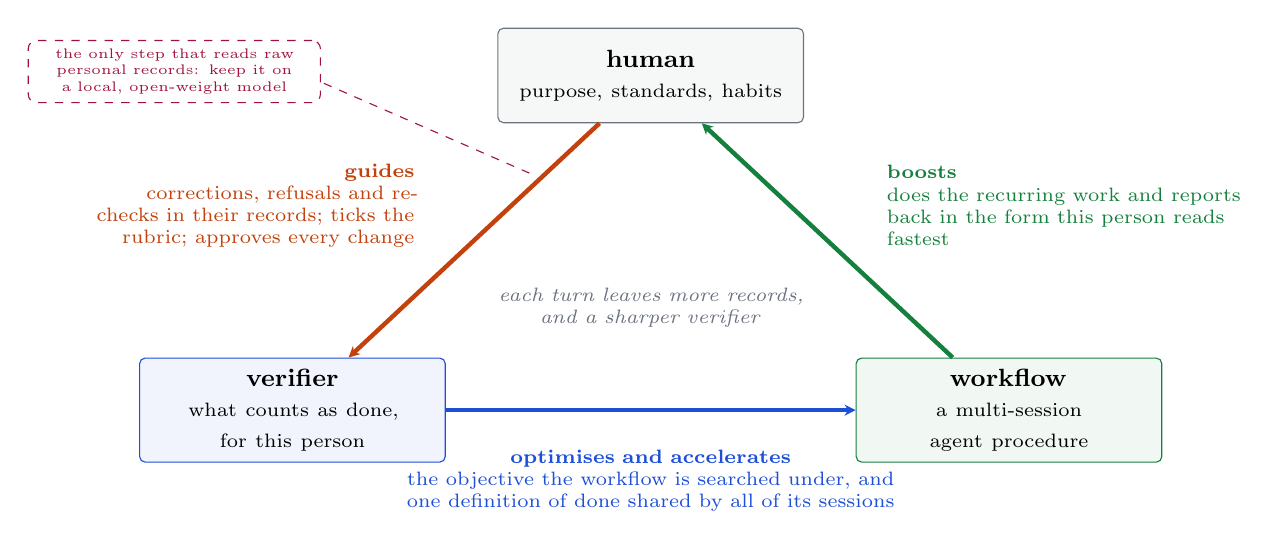
\begin{tikzpicture}[x=1cm,y=1cm]
\node[card=mainc, align=center, text width=3.6cm, minimum height=1.2cm, font=\small] (H) at (8.25,5.7) {\textbf{\T{human}{人}}\\ {\scriptsize \T{purpose, standards, habits}{目的、标准、习惯}}};
\node[card=verc, align=center, text width=3.6cm, minimum height=1.2cm, font=\small] (V) at (3.7,1.45) {\textbf{verifier}\\ {\scriptsize \T{what counts as done, for this person}{对这个人来说，怎样才算做对}}};
\node[card=wfc, align=center, text width=3.6cm, minimum height=1.2cm, font=\small] (W) at (12.8,1.45) {\textbf{workflow}\\ {\scriptsize \T{a multi-session agent procedure}{由多个 agent 会话组成的流程}}};
\draw[->, line width=1.6pt, offc] (H) -- (V);
\draw[->, line width=1.6pt, verc] (V) -- (W);
\draw[->, line width=1.6pt, wfc] (W) -- (H);
\node[align=right, font=\scriptsize, text width=4.6cm, text=offc] at (2.95,4.05) {\textbf{\T{guides}{指导}}\\ \T{corrections, refusals and re-checks in their records; ticks the rubric; approves every change}{记录里的纠正、拒绝与复核；勾选 rubric；每一次改动都由本人批准}};
\node[align=center, font=\scriptsize, text width=7cm, text=verc] at (8.25,0.55) {\textbf{\T{optimises and accelerates}{优化并加速}}\\ \T{the objective the workflow is searched under, and one definition of done shared by all of its sessions}{既是搜索 workflow 时的目标函数，也是所有会话共用的同一份“做对了”的定义}};
\node[align=left, font=\scriptsize, text width=4.6cm, text=wfc] at (13.55,4.05) {\textbf{\T{boosts}{提效}}\\ \T{does the recurring work and reports back in the form this person reads fastest}{接手重复性的工作，并按这个人读得最快的方式汇报}};
\node[note, text width=4.4cm] at (8.25,2.75) {\T{each turn leaves more records,\\ and a sharper verifier}{每转一圈，记录更多，\\ verifier 更准}};
\node[draw=hidc, dashed, rounded corners=3pt, align=center, font=\tiny, text=hidc, text width=3.5cm, inner sep=3pt] at (2.2,5.75) {\T{the only step that reads raw personal records: keep it on a local, open-weight model}{唯一会读到个人原始记录的一步：放在本地的开源模型上做}};
\draw[hidc, dashed] (4.1,5.6) -- (6.8,4.42);
\end{tikzpicture}

\caption{Why the system exists. The human guides the verifier, the verifier optimises and accelerates the workflow,
and the workflow gives the human their time back. Only the first edge touches raw personal records.}
\label{fig:triangle}
\end{figure}

Three consequences follow. Personalisation is part of the problem statement, not a feature. The verifier is the
durable asset: when a stronger model arrives the workflow can be regenerated, possibly as a completely different
procedure, while what the person accepts changes slowly. And optimisation becomes well defined: hold the
person's verifier fixed and search over workflows.

\paragraph{Where the verifier's evidence is.} It is not on the main line of the task. It is in what task mining
discards as noise: undoing and redoing, glancing back at a source without copying anything, hesitating before
sending, and, most densely, in how the person talks to their coding agents. Every ``that's wrong'', ``did you
check it?'', interrupted turn and refused tool call is an acceptance criterion stated in the person's own words,
time-stamped, with the rejected output one message above it (Figure~\ref{fig:idea}b). These logs already exist
on the machine; nothing has to be recorded.

\begin{figure}[t]
\centering
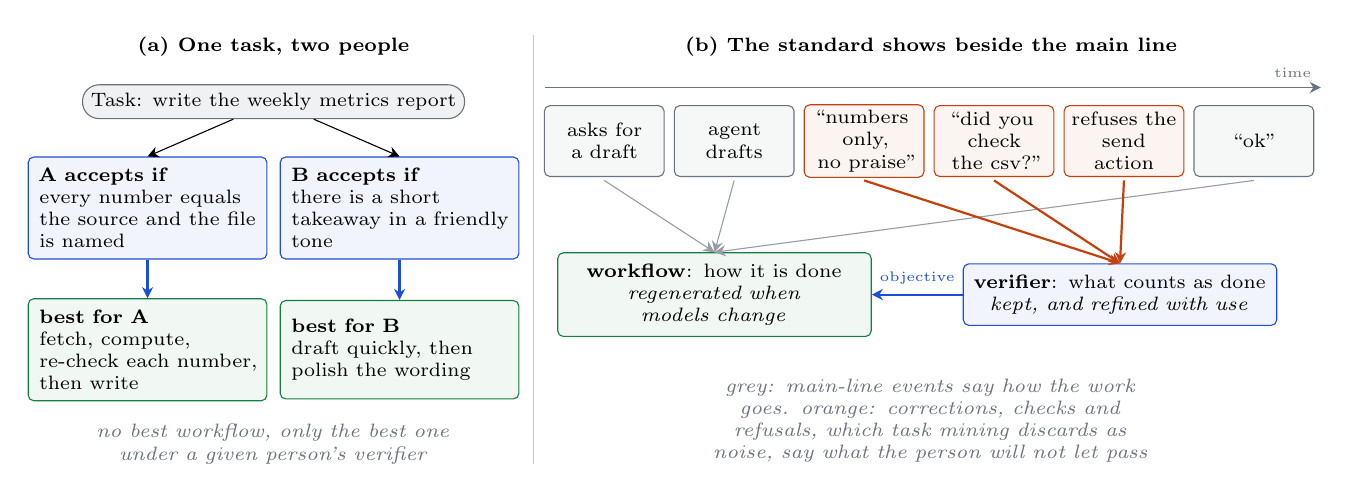
\begin{tikzpicture}[x=1cm,y=1cm]
% ---------------- (a) one task, two people
\node[lab] at (3.15,5.3) {\T{(a) One task, two people}{(a) 同一个任务，两个人}};
\node[pill] (task) at (3.15,4.6) {\T{Task: write the weekly metrics report}{任务：写每周的指标周报}};
\node[card=verc, text width=2.75cm, minimum height=1.25cm] (va) at (1.55,3.25) {\textbf{\T{A accepts if}{A 的验收标准}}\\ \T{every number equals the source and the file is named}{每个数字都与源文件一致，并写明数据来源}};
\node[card=verc, text width=2.75cm, minimum height=1.25cm] (vb) at (4.75,3.25) {\textbf{\T{B accepts if}{B 的验收标准}}\\ \T{there is a short takeaway in a friendly tone}{有一段简短的结论，语气亲切}};
\node[card=wfc, text width=2.75cm, minimum height=1.25cm] (wa) at (1.55,1.45) {\textbf{\T{best for A}{对 A 最优的做法}}\\ \T{fetch, compute, re-check each number, then write}{取数、计算、逐个核对，再动笔}};
\node[card=wfc, text width=2.75cm, minimum height=1.25cm] (wb) at (4.75,1.45) {\textbf{\T{best for B}{对 B 最优的做法}}\\ \T{draft quickly, then polish the wording}{先快速起草，再打磨措辞}};
\draw[->] (task) -- (va.north); \draw[->] (task) -- (vb.north);
\draw[->, verc, thick] (va) -- (wa); \draw[->, verc, thick] (vb) -- (wb);
\node[note, text width=6cm] at (3.15,0.25) {\T{no best workflow, only the best one\\ under a given person's verifier}{没有最优的 workflow，\\ 只有某个人的 verifier 之下的最优}};
\draw[mainc!40] (6.45,0) -- (6.45,5.45);
% ---------------- (b) where the standard shows
\node[lab] at (11.5,5.3) {\T{(b) The standard shows beside the main line}{(b) 标准出现在主线之外}};
\foreach \px/\ptxt/\pcol in {7.35/{\T{asks for\\a draft}{让 agent\\起草}}/mainc, 9.0/{\T{agent\\drafts}{agent\\起草}}/mainc,
                      10.65/{\T{``numbers only,\\no praise''}{“只要数字，\\别夸”}}/offc, 12.3/{\T{``did you check\\the csv?''}{“你核对过\\csv 吗？”}}/offc,
                      13.95/{\T{refuses the\\send action}{拒绝\\发送动作}}/offc, 15.6/{\T{``ok''}{“可以”}}/mainc}
  \node[card=\pcol, align=center, text width=1.38cm, minimum height=0.9cm, inner sep=2pt] at (\px,4.1) {\ptxt};
\draw[->, mainc] (6.6,4.78) -- (16.45,4.78) node[above left, font=\tiny, text=mainc] {\T{time}{时间}};
\node[card=wfc, text width=3.7cm, align=center] (W) at (8.75,2.15) {\textbf{workflow}\T{: how it is done}{：怎么做}\\ \emph{\T{regenerated when models change}{模型换代后可以重新生成}}};
\node[card=verc, text width=3.7cm, align=center] (V) at (13.9,2.15) {\textbf{verifier}\T{: what counts as done}{：怎样算做对}\\ \emph{\T{kept, and refined with use}{长期保留，越用越准}}};
\foreach \px in {7.35,9.0,15.6} \draw[->, mainc!70] (\px,3.6) -- (W.north);
\foreach \px in {10.65,12.3,13.95} \draw[->, offc, thick] (\px,3.6) -- (V.north);
\draw[->, verc, thick] (V) -- node[above, font=\tiny, text=verc] {\T{objective}{目标函数}} (W);
\node[note, text width=9.6cm] at (11.5,0.55) {\T{grey: main-line events say how the work goes. orange: corrections, checks and\\ refusals, which task mining discards as noise, say what the person will not let pass}{灰色：主线上的事件说明事情怎么做。橙色：纠正、核对与拒绝，\\ 也就是 task mining 当作噪声丢掉的部分，说明这个人不放过什么}};
\end{tikzpicture}

\caption{The idea. (a) The acceptance standard differs between people, and it decides which workflow is best.
(b) Evidence for that standard lies off the main line of the task, and is densest in the person's existing
conversations with coding agents.}
\label{fig:idea}
\end{figure}

\paragraph{Where this sits.} We see the automation of work with coding models as five stages
(Figure~\ref{fig:ladder}): \emph{coding}, where a person writes with a model's help; the \emph{coding agent},
where one agent carries a task from start to finish; the \emph{coding multi-agent workflow}, where several agent
sessions are arranged into a procedure; the \emph{verifier-optimised coding multi-agent workflow}, where that
arrangement is no longer made by hand but searched for under an explicit acceptance standard; and the
\emph{automated, recursively self-improving working group}, a standing group that maintains and improves its own
workflows over time. Each stage takes away one thing the person had to supply: the keystrokes, the
step-by-step supervision, the arrangement of the steps, and finally the upkeep of the arrangement. This paper
implements the fourth stage. The object that makes it possible is the same one that would make the fifth safe to
attempt: a verifier that is explicit, executable and owned by the person, so that what is being improved (the
workflow) and what judges it (the verifier) are kept apart, and a group that rewrites its own procedures still
answers to a standard it cannot rewrite on its own.

\paragraph{The next stage is about diversity.} One person's pair makes one worker in that person's image. The
working group we are aiming at is assembled from pairs distilled from \emph{many, different} people: the analyst
who will not send an unchecked number, the engineer who will not merge a fix without a regression test, the
operator who orders a queue by who asked first. Their workflows give the group a range of procedures; their
verifiers give it a range of standards that disagree in useful ways, so that work produced under one is reviewed
under another. Diversity in such a group does not have to be prompted into existence with personas: it is
inherited from the people the pairs came from, and it stays measurable, because every member's standard is an
explicit, executable object.

\paragraph{What has to stay private.} Of the three edges in Figure~\ref{fig:triangle} only one reads raw personal
records: distilling the verifier from the human. Executing a workflow sees the task at hand, and optimising it
sees the verifier, which is a short, reviewable text; neither needs the person's history. The privacy requirement
therefore falls on a single, well-delimited step, and that step is the one to run on a model the person hosts.
Samples of the kind introduced below, records paired with the style that produced them, are exactly the
supervision such a model needs, so the data set we are collecting doubles as training material for open-weight
models of a size that runs locally (the Qwen 27B and 35B-A3B class); stronger hosted models can then be used for
execution and optimisation, where nothing private is exposed.

\begin{figure}[t]
\centering
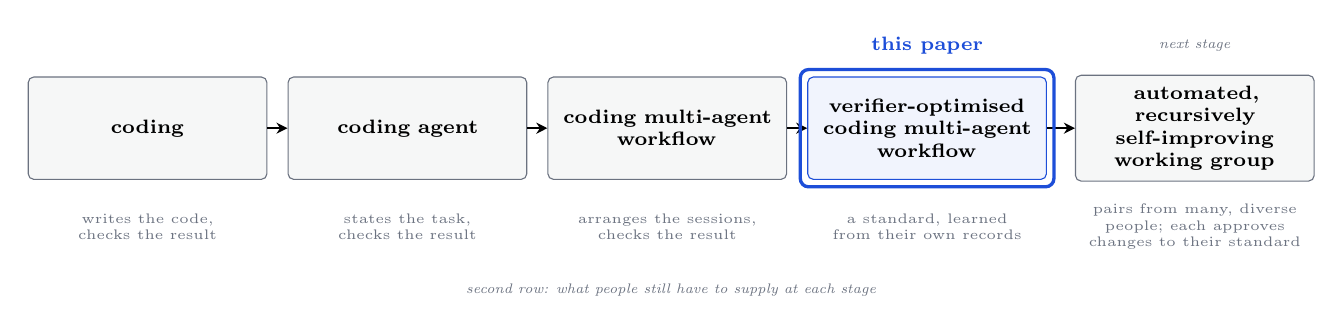
\begin{tikzpicture}[x=1cm,y=1cm]
\foreach \lk/\lx/\ltitle/\lsup/\lcol in {
   1/1.55/{\T{coding}{写代码}}/{\T{writes the code,\\checks the result}{自己写代码，\\自己检查结果}}/mainc,
   2/4.85/{coding agent}/{\T{states the task,\\checks the result}{说明任务，\\检查结果}}/mainc,
   3/8.15/{\T{coding multi-agent\\workflow}{coding 多 agent\\workflow}}/{\T{arranges the sessions,\\checks the result}{编排各个会话，\\检查结果}}/mainc,
   4/11.45/{\T{verifier-optimised\\coding multi-agent\\workflow}{由 verifier 优化的\\coding 多 agent\\workflow}}/{\T{a standard, learned\\from their own records}{一份标准，\\从本人的记录里学出来}}/verc,
   5/14.85/{\T{automated, recursively\\self-improving\\working group}{自动化、递归自我\\改进的\\working group}}/{\T{pairs from many, diverse\\people; each approves\\changes to their standard}{来自许多不同的人的\\(workflow, verifier)；\\各自批准自己标准的改动}}/mainc}
{
  \node[card=\lcol, align=center, text width=2.75cm, minimum height=1.3cm] (L\lk) at (\lx,1.7) {\textbf{\ltitle}};
  \node[font=\tiny, text=mainc, align=center] at (\lx,0.45) {\lsup};
}
\foreach \lk [evaluate=\lk as \lnext using int(\lk+1)] in {1,...,4} \draw[->, thick] (L\lk.east) -- (L\lnext.west);
\node[draw=verc, very thick, rounded corners=3pt, fit=(L4), inner sep=2.5pt] {};
\node[font=\scriptsize\bfseries, text=verc] at (11.45,2.75) {\T{this paper}{本文}};
\node[font=\tiny\itshape, text=mainc] at (14.85,2.75) {\T{next stage}{下一阶段}};
\node[font=\tiny\itshape, text=mainc] at (8.2,-0.35) {\T{second row: what people still have to supply at each stage}{第二行：每个阶段仍然需要人来提供的东西}};
\end{tikzpicture}

\caption{The trajectory we have in mind. Each stage removes something the person had to supply. This work is the
fourth stage: the multi-session workflow is optimised against a verifier learned from the person's records. The
fifth assembles pairs distilled from many different people into one group.}
\label{fig:ladder}
\end{figure}

\paragraph{Contributions.}
\begin{itemize}
\item A formulation of personal automation as a human--verifier--workflow triangle in which the object to learn is
      a pair (workflow, verifier), with a verifier in five layers
      (objective, process, style, preference, report) plus a checking policy (\S\ref{sec:method}).
\item \sys{}, an open implementation that reads access records a person already has under per-source consent,
      calls no model API itself, and delegates all reading and writing to headless sessions of an existing coding
      agent whose outputs it constrains with deterministic checks.
\item A sample format and scoring protocol with a hidden, pre-filled personal style, including an order-sensitive,
      seven-day stateful task, and first measurements on six samples (\S\ref{sec:bench}--\ref{sec:results}).
\end{itemize}

% ---------------------------------------------------------------------------------------------------------------
\section{Problem}
\label{sec:problem}

A person $u$ leaves \emph{access records} $R_u$: conversations with coding agents, shell history, browser history,
exported chats, file names and modification times, optionally screen recordings. For a recurring task the person
has a \emph{purpose} and can state a short \emph{rubric} $Q_u$, the items they would tick off. Behind it is a larger
\emph{style} $S_u$: standards they apply but rarely state, about results, about the order in which things are done,
and about how results are reported back to them.

From $R_u$ and $Q_u$ the system produces
\begin{itemize}
\item a \emph{workflow} $W$: an ordered list of prompts, one per agent session; sessions share no memory and hand
      over through files;
\item a \emph{verifier} $V$: a set of items, each a claim with either an executable check or a judging rubric, a
      layer, a weight, and pointers to the records that justify it; and a \emph{policy} describing how this person
      checks (how deep, when, what to do on failure, when to stop and ask).
\end{itemize}
$V$ is rendered into a single prompt that every session of $W$ receives, so the procedure may be cut into any
number of sessions but there is one definition of done.

We measure three things on a held-out instance of the task with reference output $y^\star$ (what $u$ would keep):
\begin{align*}
\textbf{rubric completion} &:\quad |\{q \in Q_u : q(W(x)) \text{ holds}\}| \,/\, |Q_u|, \\
\textbf{style coverage} &:\quad |\{s \in S_u : V \text{ fails } y^\star_{\neg s} \text{ on an item it passes on } y^\star\}| \,/\, |S_u|,\\
\textbf{reference acceptance} &:\quad V(y^\star) = \text{accept},
\end{align*}
where $y^\star_{\neg s}$ is the reference broken in exactly the way $s$ forbids. Coverage rewards a strict
verifier; reference acceptance penalises one that is strict about the wrong things. For long-horizon tasks rubric
completion is reported per day, and the headline number is how many days are \emph{filled}, i.e.\ pass every
applicable rubric item.

% ---------------------------------------------------------------------------------------------------------------
\section{An example: a week of refunds}
\label{sec:example}

Figure~\ref{fig:week} shows our hardest sample. Xu~Qing handles after-sale refunds for a small shop. Each day she
receives a sheet of refund requests and works through them in a back office where every action is real: a refund
cannot be undone, and neither can a notification to the buyer. The back office allows at most \textyen 1000 of
refunds per day and declines anything beyond that.

What the system is given is short: the purpose, a rubric of seven items (results equal hers; every order is looked
up before anything is done to it; the buyer is notified once, last; nothing declined or refunded twice; the report's
first line states the day's totals; on Sunday a week summary), and her access records: about sixty agent turns,
twenty-three shell commands, twenty-three chat messages and five page visits, roughly half of them unrelated.

What it is not given are the seventeen standards from which those records were written. Six govern order and
gating within a day (oldest request first, not sheet order; a buyer-caused return loses the shipping fee; above
\textyen 500 escalate; refund before notifying; no refund until the return is signed for; never split a refund to
fit the cap). Five govern how she wants to be told (verdict in the first line; one row per order, no narration;
what needs her at the top, marked; amounts as \textyen{} with two decimals; no logs). Six only exist across days
(yesterday's unpaid orders join today's queue by their original request time; an approved order is refunded the
day it is approved; a re-request after a completed return is not a duplicate; a re-request after a refund is; a
rejection is told to the buyer; the week summary follows the same reporting rule).

\begin{figure}[t]
\centering
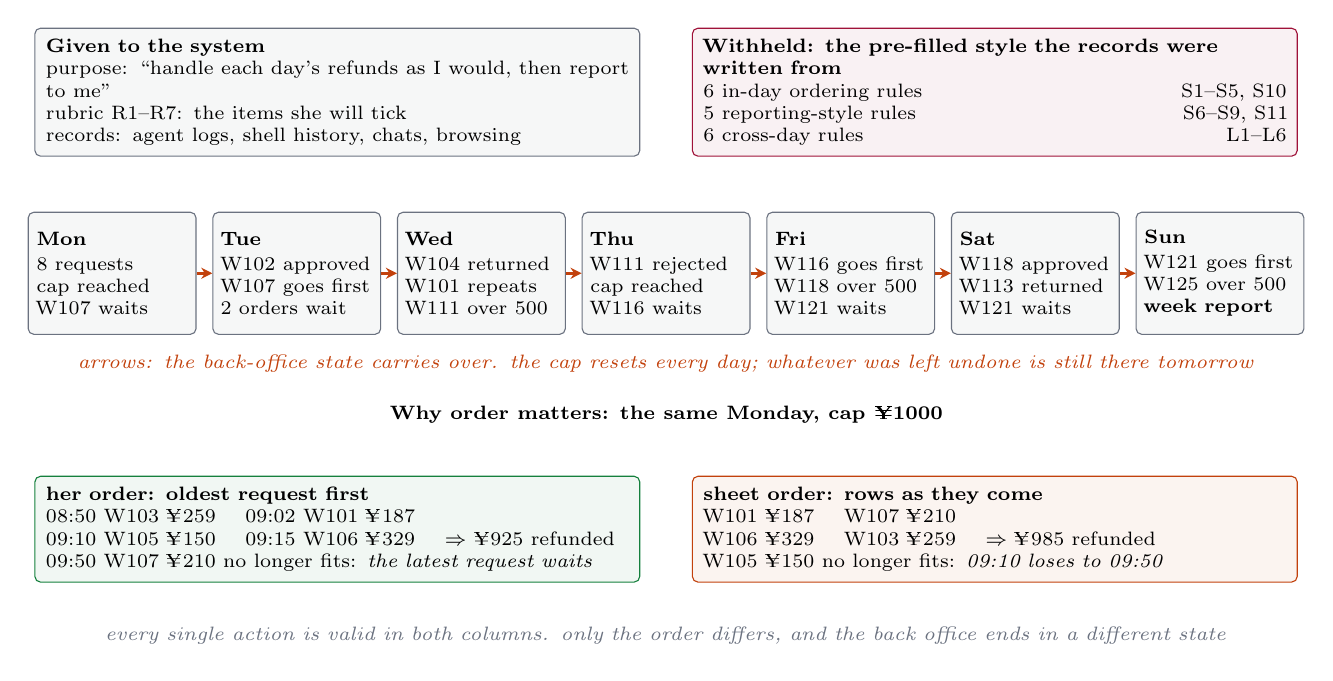
\begin{tikzpicture}[x=1cm,y=1cm]
% visible / hidden
\node[card=mainc, text width=7.4cm] (vis) at (4.0,7.75) {\textbf{\T{Given to the system}{给系统看的}}\\
\T{purpose: ``handle each day's refunds as I would, then report to me''}{目的：“每天的退款按我的做法处理完，再向我汇报”}\\
\T{rubric R1--R7: the items she will tick}{rubric R1--R7：她会逐条勾的验收项}\\
\T{records: agent logs, shell history, chats, browsing}{记录：agent 对话、shell 历史、聊天、浏览}};
\node[card=hidc, text width=7.4cm] (hid) at (12.35,7.75) {\textbf{\T{Withheld: the pre-filled style the records were written from}{隐藏的：预先填好、用来生成这些记录的个人风格}}\\
\T{6 in-day ordering rules}{6 条当天内的顺序规则} \hfill S1--S5, S10\\
\T{5 reporting-style rules}{5 条汇报风格} \hfill S6--S9, S11\\
\T{6 cross-day rules}{6 条跨天规则} \hfill L1--L6};
% days
\foreach \dk/\dn/\dtxt in {0/{\T{Mon}{周一}}/{\T{8 requests\\cap reached\\W107 waits}{8 条申请\\额度用完\\W107 等明天}},
                      1/{\T{Tue}{周二}}/{\T{W102 approved\\W107 goes first\\2 orders wait}{W102 获批\\W107 排最前\\2 单等明天}},
                      2/{\T{Wed}{周三}}/{\T{W104 returned\\W101 repeats\\W111 over 500}{W104 已寄回\\W101 重复申请\\W111 超 500}},
                      3/{\T{Thu}{周四}}/{\T{W111 rejected\\cap reached\\W116 waits}{W111 被驳回\\额度用完\\W116 等明天}},
                      4/{\T{Fri}{周五}}/{\T{W116 goes first\\W118 over 500\\W121 waits}{W116 排最前\\W118 超 500\\W121 等明天}},
                      5/{\T{Sat}{周六}}/{\T{W118 approved\\W113 returned\\W121 waits}{W118 获批\\W113 已寄回\\W121 继续等}},
                      6/{\T{Sun}{周日}}/{\T{W121 goes first\\W125 over 500\\\textbf{week report}}{W121 排最前\\W125 超 500\\\textbf{周汇总}}}}
  \node[card=mainc, text width=1.92cm, minimum height=1.55cm, inner sep=3pt] (day\dk) at (\dk*2.345+1.14,5.45) {\textbf{\dn}\\[1pt] \dtxt};
\foreach \dk [evaluate=\dk as \dnext using int(\dk+1)] in {0,...,5}
  \draw[->, offc, very thick] (day\dk.east) -- (day\dnext.west);
\node[note, text=offc, text width=15.5cm] at (8.18,4.3) {\T{arrows: the back-office state carries over. the cap resets every day; whatever was left undone is still there tomorrow}{箭头：后台状态延续到第二天。额度每天重置；没办完的事明天还在}};
% order matters
\node[lab] at (8.18,3.65) {\T{Why order matters: the same Monday, cap \textyen 1000}{为什么顺序要紧：同一个周一，额度 \textyen 1000}};
\node[card=wfc, text width=7.4cm] (good) at (4.0,2.2) {\textbf{\T{her order: oldest request first}{她的顺序：先申请的先处理}}\\
08:50 W103 \textyen 259 \quad 09:02 W101 \textyen 187\\
09:10 W105 \textyen 150 \quad 09:15 W106 \textyen 329 \quad $\Rightarrow$ \T{\textyen 925 refunded}{共退 \textyen 925}\\
\T{09:50 W107 \textyen 210 no longer fits: \emph{the latest request waits}}{09:50 的 W107 \textyen 210 放不下：\emph{最晚申请的等明天}}};
\node[card=offc, text width=7.4cm] (bad) at (12.35,2.2) {\textbf{\T{sheet order: rows as they come}{表格顺序：按行处理}}\\
W101 \textyen 187 \quad W107 \textyen 210\\
W106 \textyen 329 \quad W103 \textyen 259 \quad $\Rightarrow$ \T{\textyen 985 refunded}{共退 \textyen 985}\\
\T{W105 \textyen 150 no longer fits: \emph{09:10 loses to 09:50}}{W105 \textyen 150 放不下：\emph{09:10 申请的输给了 09:50 的}}};
\node[note, text width=15.5cm] at (8.18,0.85) {\T{every single action is valid in both columns. only the order differs, and the back office ends in a different state}{两边的每一个动作单看都合法，只有顺序不同，后台的最终状态却不一样}};
\end{tikzpicture}

\caption{The seven-day sample. Top: what the system sees and what is withheld. Middle: the week; orders that could
not be paid, approvals and returned parcels connect the days. Bottom: the same Monday handled in two orders.}
\label{fig:week}
\end{figure}

The task is built so that a correct-looking workflow in the wrong order fails. The bottom of
Figure~\ref{fig:week} shows Monday. Handled by request time, four orders are refunded and the latest request
waits for tomorrow's cap. Handled in sheet order, every individual action is still legitimate, but a later request
consumes the cap and an earlier one is turned away; the back office ends in a different state, and on Tuesday a
different order is at the head of the queue. The reference week and every process probe are produced by actually
running the back office, once following her rules and once per rule with that rule ignored, so that journal, state
and report remain mutually consistent: a verifier can only catch a probe by knowing the rule.

% ---------------------------------------------------------------------------------------------------------------
\section{Method}
\label{sec:method}

\begin{figure}[t]
\centering

\resizebox{\textwidth}{!}{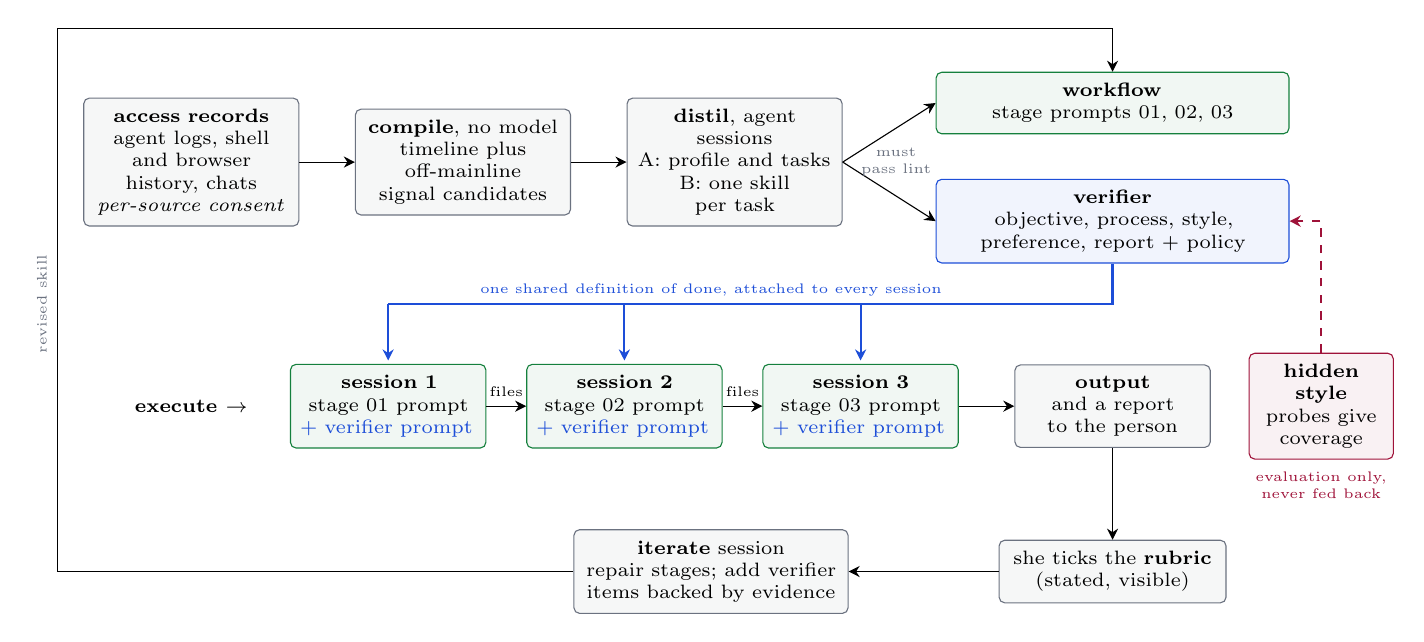
\begin{tikzpicture}[x=1cm,y=1cm]
% row 1: pipeline
\node[card=mainc, text width=2.45cm, align=center] (rec) at (1.4,6.3) {\textbf{\T{access records}{访问记录}}\\ \T{agent logs, shell and browser history, chats}{agent 对话、shell 与浏览器历史、聊天}\\ \emph{\T{per-source consent}{逐项授权}}};
\node[card=mainc, text width=2.45cm, align=center] (cmp) at (4.85,6.3) {\textbf{\T{compile}{编译}}\T{, no model}{（不调模型）}\\ \T{timeline plus off-mainline signal candidates}{时间线 + 主线之外的信号候选}};
\node[card=mainc, text width=2.45cm, align=center] (dst) at (8.3,6.3) {\textbf{\T{distil}{蒸馏}}\T{, agent sessions}{（agent 会话）}\\ \T{A: profile and tasks}{A：画像与任务}\\ \T{B: one skill per task}{B：每个任务一个 skill}};
\node[card=wfc, text width=4.2cm, align=center] (wf) at (13.1,7.05) {\textbf{workflow}\\ \T{stage prompts 01, 02, 03}{各阶段的 prompt：01、02、03}};
\node[card=verc, text width=4.2cm, align=center] (vf) at (13.1,5.55) {\textbf{verifier}\\ \T{objective, process, style,\\ preference, report $+$ policy}{客观、顺序、风格、偏好、汇报\\ $+$ 检查方式}};
\draw[->] (rec) -- (cmp); \draw[->] (cmp) -- (dst);
\draw[->] (dst.east) -- (wf.west); \draw[->] (dst.east) -- (vf.west);
\node[font=\tiny, text=mainc, align=center] at (10.35,6.3) {\T{must\\pass lint}{须通过\\lint}};
% row 2: execution
\node[lab] at (1.4,3.2) {\T{execute}{执行} $\rightarrow$};
\foreach \sk/\sx in {1/3.9,2/6.9,3/9.9}
  \node[card=wfc, text width=2.2cm, align=center] (s\sk) at (\sx,3.2) {\textbf{\T{session}{会话} \sk}\\ \T{stage 0\sk{} prompt}{阶段 0\sk{} 的 prompt}\\ \textcolor{verc}{$+$ \T{verifier prompt}{verifier 的 prompt}}};
\node[card=mainc, text width=2.2cm, align=center] (out) at (13.1,3.2) {\textbf{\T{output}{产出}}\\ \T{and a report\\ to the person}{以及给本人的\\ 汇报}};
\draw[->] (s1) -- node[above, font=\tiny] {\T{files}{文件}} (s2); \draw[->] (s2) -- node[above, font=\tiny] {\T{files}{文件}} (s3); \draw[->] (s3) -- (out);
\draw[verc, thick] (vf.south) -- (13.1,4.5) -- (3.9,4.5);
\foreach \sx in {3.9,6.9,9.9} \draw[->, verc, thick] (\sx,4.5) -- (\sx,3.78);
\node[font=\tiny, text=verc] at (8.0,4.68) {\T{one shared definition of done, attached to every session}{同一份“做对了”的定义，附给每一个会话}};
% row 3: signals
\node[card=mainc, text width=2.6cm, align=center] (fb) at (13.1,1.1) {\T{she ticks the \textbf{rubric}\\ (stated, visible)}{本人勾 \textbf{rubric}\\ （说出口的、可见的）}};
\node[card=mainc, text width=3.2cm, align=center] (it) at (8.0,1.1) {\T{\textbf{iterate} session\\ repair stages; add verifier\\ items backed by evidence}{\textbf{迭代}会话\\ 修各阶段；补上有证据的\\ 验收条目}};
\node[card=hidc, text width=1.55cm, align=center] (pr) at (15.75,3.2) {\textbf{\T{hidden style}{隐藏风格}}\\ \T{probes give coverage}{探针给出覆盖率}};
\draw[->] (out) -- (fb);
\draw[->] (fb) -- (it);
\draw[->] (it.west) -- (-0.3,1.1) -- (-0.3,8.0) -- (13.1,8.0) -- (wf.north);
\node[font=\tiny, text=mainc, rotate=90] at (-0.5,4.5) {\T{revised skill}{修订后的 skill}};
\draw[->, hidc, dashed, thick] (pr.north) -- (15.75,5.55) -- (vf.east);
\node[font=\tiny, text=hidc, align=center] at (15.75,2.2) {\T{evaluation only,\\never fed back}{只用于评测，\\从不反馈}};
\end{tikzpicture}
}
\caption{The pipeline. Records are collected under consent and compressed without a model; agent sessions distil
a profile and, per task, a workflow and a verifier; the workflow runs as several sessions that all receive the
verifier as the same prompt. Rubric failures drive revisions. Hidden style items are used only for scoring.}
\label{fig:method}
\end{figure}

\paragraph{Collect, with consent.} Each source is discovered without being opened and is read only after the
person allows it: local and remote coding-agent logs, shell history, browser history (host and path only),
exported chats, recently opened files, git commits. Screen recording and video import are optional extras. All
text is redacted before storage. Every source writes the same event format.

\paragraph{Compile, without a model.} A day of events becomes a timeline and a list of \emph{off-mainline signal
candidates}. Conversation signals need only logs: a correction after an agent reply, a request for proof, an
interrupted turn, a refused tool call, a user-authored task specification. Screen signals need recording: a
glance at another window that copies nothing back (a cross-check, as opposed to a look-up that does), undo
bursts, a file saved again after the person had moved on (which yields a rejected and a kept version of the same
artefact without any labelling). Detectors are deliberately high-recall; each hit is a pointer for the agent to
interpret, not a conclusion.

\paragraph{Distil, in someone else's agent.} \sys{} calls no model API. It writes a task brief (outputs, hard
constraints, stop conditions, self-check) and opens a headless session in an installed coding agent. One session
writes a profile, the person's working habits, acceptance style, reporting style and ordering habits, each with
evidence, and lists candidate tasks. One session per task then writes the skill.

\paragraph{The pair.} The workflow is a sequence of stage prompts. The verifier has five layers:
\emph{objective} (person-independent correctness), \emph{process} (order and gating of actions, checked on the
journal an execution leaves), \emph{style} (this person, across tasks), \emph{preference} (this person, this task)
and \emph{report} (structure, length and readability of what is reported back). Every personal item must cite
records or be marked a low-confidence hypothesis. A lint step rejects a verifier that fails outputs the person
kept, or that has nothing able to fail outputs the person discarded.

\paragraph{Execute and revise.} Each stage runs as its own session; the verifier prompt is appended to all of
them, and the last stage runs the executable checks. After a run the person's rubric verdicts go to an
\emph{iterate} session that may repair stages and add evidence-backed verifier items. In the optimisation loop
proper the verifier is frozen by hash while the workflow is revised, the reviser never sees held-out results, and
a change to the verifier takes effect only after the person approves it.

% ---------------------------------------------------------------------------------------------------------------
\section{Samples with a hidden style}
\label{sec:bench}

A sample is built in the order a person exists: first the style, then the behaviour. We write a persona, a
purpose, a rubric and a list of style items; we then write access records in which each style item leaves the
kind of trace it would naturally leave (a pushed-back draft, a question about whether something was checked, a
remark to a colleague, a refused action), mixed with unrelated activity. Records are rendered into each source's
native format (agent session logs, time-stamped shell history, a browser history database, a chat export) and
read back by the real collectors. The style list and the reference output are withheld. A validity check requires
that every style item conditions at least one record and that the reference passes the sample's own rubric.
Table~\ref{tab:samples} lists the six samples.

\begin{table}[h]
\centering\footnotesize\setlength{\tabcolsep}{4pt}
\begin{tabular}{@{}llllcc@{}}
\toprule
sample & person & task & record sources & hidden items & horizon \\
\midrule
weekly-report & growth analyst & two csv files $\rightarrow$ report & 2 agents, shell, web, chat & 7 & 1 step \\
swe-bugfix & backend engineer & issue $\rightarrow$ fix, test, commit msg & agent, shell, web, chat & 7 & 1 step \\
guest-reply & guesthouse owner & guest message $\rightarrow$ reply & agent, web, chat & 7 & 1 step \\
video-publish & cooking vlogger & shoot notes $\rightarrow$ publish metadata & agent, web, chat & 7 & 1 step \\
refund-ops & after-sale operator & one day of refunds, stateful & agent, shell, web, chat & 11 & 1 day \\
refund-week & after-sale operator & seven days of refunds, stateful & agent, shell, web, chat & 17 & 7 days \\
\bottomrule
\end{tabular}
\caption{Samples. In the two refund samples the order of actions changes the final state.}
\label{tab:samples}
\end{table}

% ---------------------------------------------------------------------------------------------------------------
\section{First results}
\label{sec:results}

\paragraph{Setup.} All sessions are Codex CLI sessions with \texttt{gpt-6-astra} at \texttt{xhigh} reasoning
effort on one server. Each sample was run once. For the single-step samples we run the built skill, give the
rubric verdicts to one iterate session, and run again; judged verifier items are evaluated only in the last round.

\begin{table}[h]
\centering\small
\begin{tabular}{@{}lccccc@{}}
\toprule
 & \multicolumn{2}{c}{rubric completion} & \multicolumn{2}{c}{style coverage} & reference \\
\cmidrule(lr){2-3}\cmidrule(lr){4-5}
sample & round 0 & round 1 & checks only & with judged items & accepted \\
\midrule
weekly-report & 5/5 & 5/5$^{\dagger}$ & 6/6 & 6/6 & yes \\
swe-bugfix    & 4/5 & 5/5 & 1/6 & 6/6 & \textbf{no} \\
guest-reply   & 5/5 & 4/5 & 4/6 & 6/6 & \textbf{no} \\
video-publish & 5/5 & 5/5 & 5/6 & 6/6 & yes \\
\bottomrule
\end{tabular}
\caption{Single-step samples, one run each. One hidden item per sample is a process standard without an output
probe and is not scored. $^{\dagger}$Originally scored 2/5 because one of our rubric items wrongly required list
bullets; the value shown is the same output re-scored after correcting the rubric.}
\label{tab:single}
\end{table}

\paragraph{Single-step tasks are too easy.} Three of four workflows satisfy the whole rubric on the first
execution, and all hidden items with a probe are caught once judged items are evaluated
(Table~\ref{tab:single}). In these samples the output is one static file, the order of work does not matter, and
each standard was stated almost verbatim by the person in a conversation. They validate the plumbing and little
else, which is why the refund samples were built.

\paragraph{Coverage alone is misleading.} For two of the four samples the verifier produced after one revision
\emph{rejects the reference output}, the reply or patch the person would have kept. In \emph{guest-reply} the
revised verifier fails the reference on three hard items: that the stated early check-in fee omits the condition
``subject to availability'', that the quoted total does not include the pet fee, and that the output carries no
execution record proving the reply was not sent. Each is defensible in isolation and none is hers. The same
revision made the workflow so cautious that it wrote a block notice next to a correct reply and lost a rubric item
it had satisfied before. A verifier that fails everything would score full coverage; reference acceptance has to
be reported with it, and the revision step needs the person's kept outputs as a regression set.

\paragraph{Scoring artefacts are easy to introduce.} The apparent drop of \emph{weekly-report} from 5/5 to 2/5
was ours: the rubric demanded list bullets the person never asked for. We keep the incident in the table because
it is the same failure as the previous paragraph on the benchmark's side, an over-specific check standing in for
a standard.

\paragraph{The week.} \todo{refund-week result: days filled out of 7, per-day rubric matrix, style coverage by
group (in-day order / reporting / cross-day), reference acceptance per day. Run in progress at the time of writing;
fill in from \texttt{bench-report.md}.}

\paragraph{Caveats.} These numbers are from one run, one model and samples whose records we wrote ourselves to
express the style, so they are closer to an upper bound than to an estimate. There are no human participants yet.
The system has not been run end to end on a real person's records with an agent backend; on the author's machine
only the deterministic stages have been exercised on real logs.

% ---------------------------------------------------------------------------------------------------------------
\section{Related work}
\label{sec:related}

\emph{Demonstration to skill.} Products now turn one recorded, sometimes narrated, demonstration into a reusable
skill~\cite{recordskill,recordreplay,skillrecorder}. They are single-shot, need the person to perform, and record
the main line. \emph{Passive traces to task and user models.} Task model induction~\cite{tmi} separates
interleaved tasks in unlabeled traces and builds goal hierarchies with control flow; general user
models~\cite{gum} maintain confidence-weighted propositions about a user from screenshots. Neither produces
acceptance criteria. A study of mining skill files from GUI trajectories reports readable clusters with little
downstream benefit~\cite{skillmd}, which we read as the absence of an objective. \emph{Workflows from agent
trajectories}~\cite{awm} take success from a benchmark evaluator. \emph{Skills with verifiers.}
EvoSkills~\cite{evoskills} co-evolves a skill generator and a surrogate verifier and reports large losses without
the verifier; agentic rubrics~\cite{rubrics} have an agent write a weighted checklist from a repository. Their
verifiers are derived from the task, not from a person. \emph{Preferences from implicit feedback.}
PRELUDE~\cite{prelude} infers latent preferences from a user's edits to agent output and uses them to condition
generation. We extend the signal from edits to corrections, refusals and ordering habits, and use the result as
an executable acceptance test. \todo{This section relies on abstracts and secondary summaries; verify each claim
against the papers before submission.}

% ---------------------------------------------------------------------------------------------------------------
\section{Limitations and next steps}

Neither the diverse working group nor local distillation exists yet: no open-weight model has been trained or
evaluated on the samples, and all sessions reported here ran on a hosted model. The central claim, that a
workflow optimised under another person's verifier is accepted less often, is not yet tested; it needs two people (or two styles over the same task) and a cross-evaluation. The synthetic records are
kinder than real ones: the person states most standards outright, and little contradicts them. Harder samples
should include standards that are only ever shown, never said; standards that change over time; and colleagues
whose different habits appear in the same chats (the refund samples contain a few). Isolation of held-out material
relies on working directories, not on an operating-system sandbox. Finally, the verifier is only as good as the
person's own blind spots; the objective layer and the visibility of every item are the current answer to that.

\begin{thebibliography}{9}\small
\bibitem{recordskill} Anthropic. Record a Skill in Claude Cowork. Product feature, 2026.
\bibitem{recordreplay} OpenAI. Record \& Replay in the Codex desktop app. Product feature, 2026.
\bibitem{skillrecorder} Microsoft. Skill Recorder. \url{https://github.com/microsoft/skill-recorder}, 2026.
\bibitem{tmi} Y.~Jiang, Z.~Z.~Wang, R.~Chen, D.~Yang. Inducing Task Models from Computer-Use Traces. arXiv:2608.20319, 2026.
\bibitem{gum} O.~Shaikh et al. Creating General User Models from Computer Use. arXiv:2505.10831, 2025.
\bibitem{skillmd} Mining skill files from GUI trajectories. arXiv:2606.20363, 2026. \todo{authors, exact title}
\bibitem{awm} Z.~Z.~Wang et al. Agent Workflow Memory. arXiv:2409.07429, 2024.
\bibitem{evoskills} EvoSkills: co-evolving skills and surrogate verifiers. arXiv:2604.01687, 2026. \todo{authors, exact title}
\bibitem{rubrics} Agentic Rubrics as Contextual Verifiers for SWE Agents. arXiv:2601.04171, 2026. \todo{authors}
\bibitem{prelude} G.~Gao, A.~Taymanov, E.~Salinas, P.~Mineiro, D.~Misra. Aligning LLM Agents by Learning Latent Preference from User Edits. NeurIPS, 2024.
\end{thebibliography}

\end{document}
